% Appendix Template

\chapter{Nested Comments Grammar} % Main appendix title

\label{app:comments} % Change X to a consecutive letter; for referencing this appendix elsewhere, use \ref{AppendixX}

\section{Original definition} \label{app:comments:contexts}
\lstinputlisting[language=RascalGrammar, caption={A grammar showing nested comments}]{Code/grammars/comments/comments.grammar}

\section{Simplified without priority} \label{app:comments:simple}
\lstinputlisting[language=RascalGrammar, caption={The same grammar but simplified with priority removal}]{Code/grammars/comments/plain.grammar}

\section{Strongly Regular} \label{app:comments:stronglyregular}
\lstinputlisting[language=RascalGrammar, caption={The strongly regular approximation of the original grammar}]{Code/grammars/comments/StronglyRegular.grammar}

\pagebreak\subsection{NFA for strongly regular Comment}
\begin{figure}[h!]
	\centering
	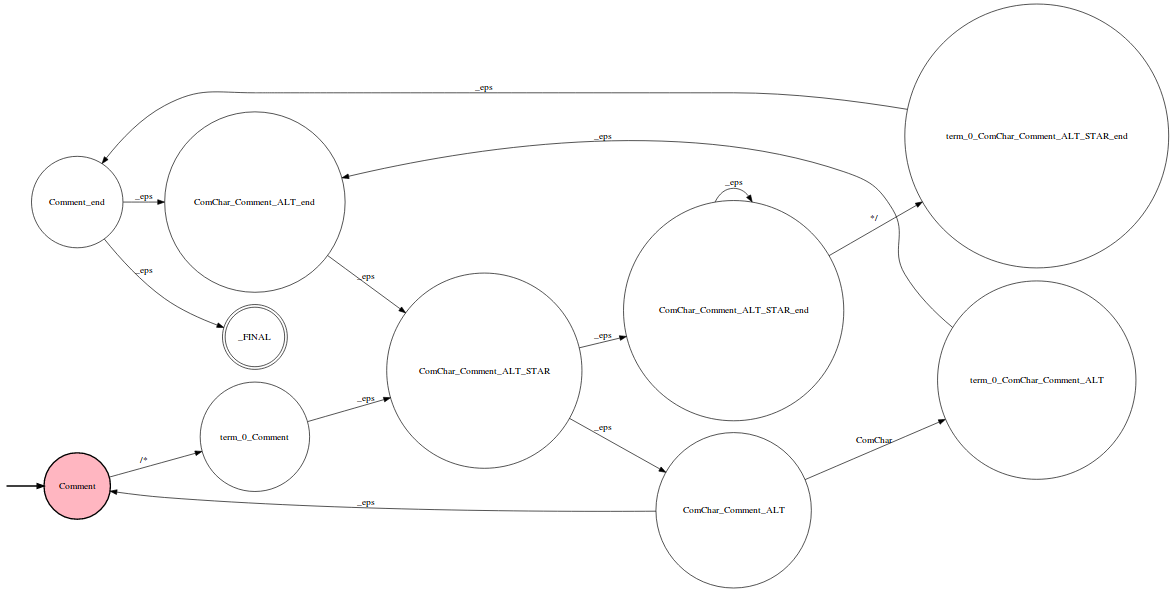
\includegraphics[width=\textwidth, keepaspectratio]{Figures/comment_nfa.png}
	\decoRule
 	\caption[NFA for Comment]{The NFA for Comment, produced from the strongly regular approximation}
 	\label{fig:comments:NFA:Comment}
\end{figure}

\subsection{DFA for strongly regular Comment}
\begin{figure}[h!]
	\centering
	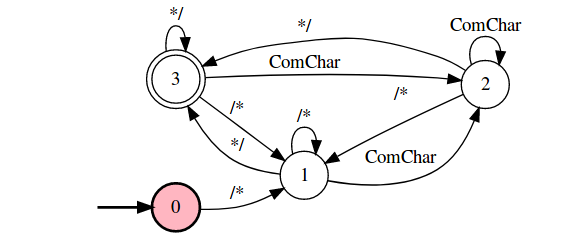
\includegraphics[width=\textwidth, keepaspectratio]{Figures/comment_dfa.png}
	\decoRule
 	\caption[DFA for Comment]{The DFA for Comment, produced from the strongly regular approximation}
 	\label{fig:comments:DFA:Comment}
\end{figure}

\pagebreak\subsection{Results of generated highlighter}
\begin{figure}[h!]
	\centering
	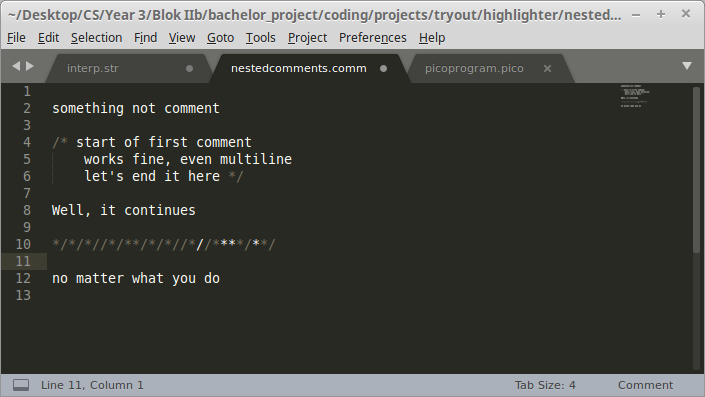
\includegraphics[width=\textwidth, keepaspectratio]{Figures/highlightShots/comment_generated.png}
	\decoRule
 	\caption[generated highlighter results for NestedComments grammar]{Results of the generated highlighter for this grammar}
 	\label{fig:comments:highlighter:generated}
\end{figure}

\subsection{Results of hand-written highlighter}
\begin{figure}[h!]
	\centering
	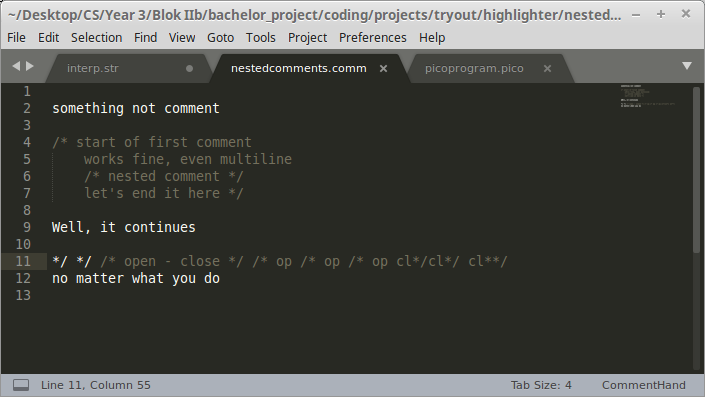
\includegraphics[width=\textwidth, keepaspectratio]{Figures/highlightShots/comment_handwritten.png}
	\decoRule
 	\caption[Hand-written highlighter results for NestedComments grammar]{Results of hand-written highlighter for this grammar}
 	\label{fig:comments:highlighter:written}
\end{figure}
